\subsection{شبیه‌سازی کانال رول استند سه درجه أزادی در حضور کنترل‌کننده \lr{LQR}}\label{roll_lqr_section_simulation}
در بخش
\ref{quadchanell_roll}
شبیه‌سازی کانال رول استند چهارپره انجام شد. در این بخش به بررسی عملکرد چهارپره در حضور کنترل‌کننده \lr{LQR} پرداخته می‌شود. در شبیه‌سازی برای بهینه‌سازی ضرایب وزنی \lr{LQR} از روش
\lr{TCACS} \cite{Karimi2010}
استفاده شده است.
\begin{figure}[H]
	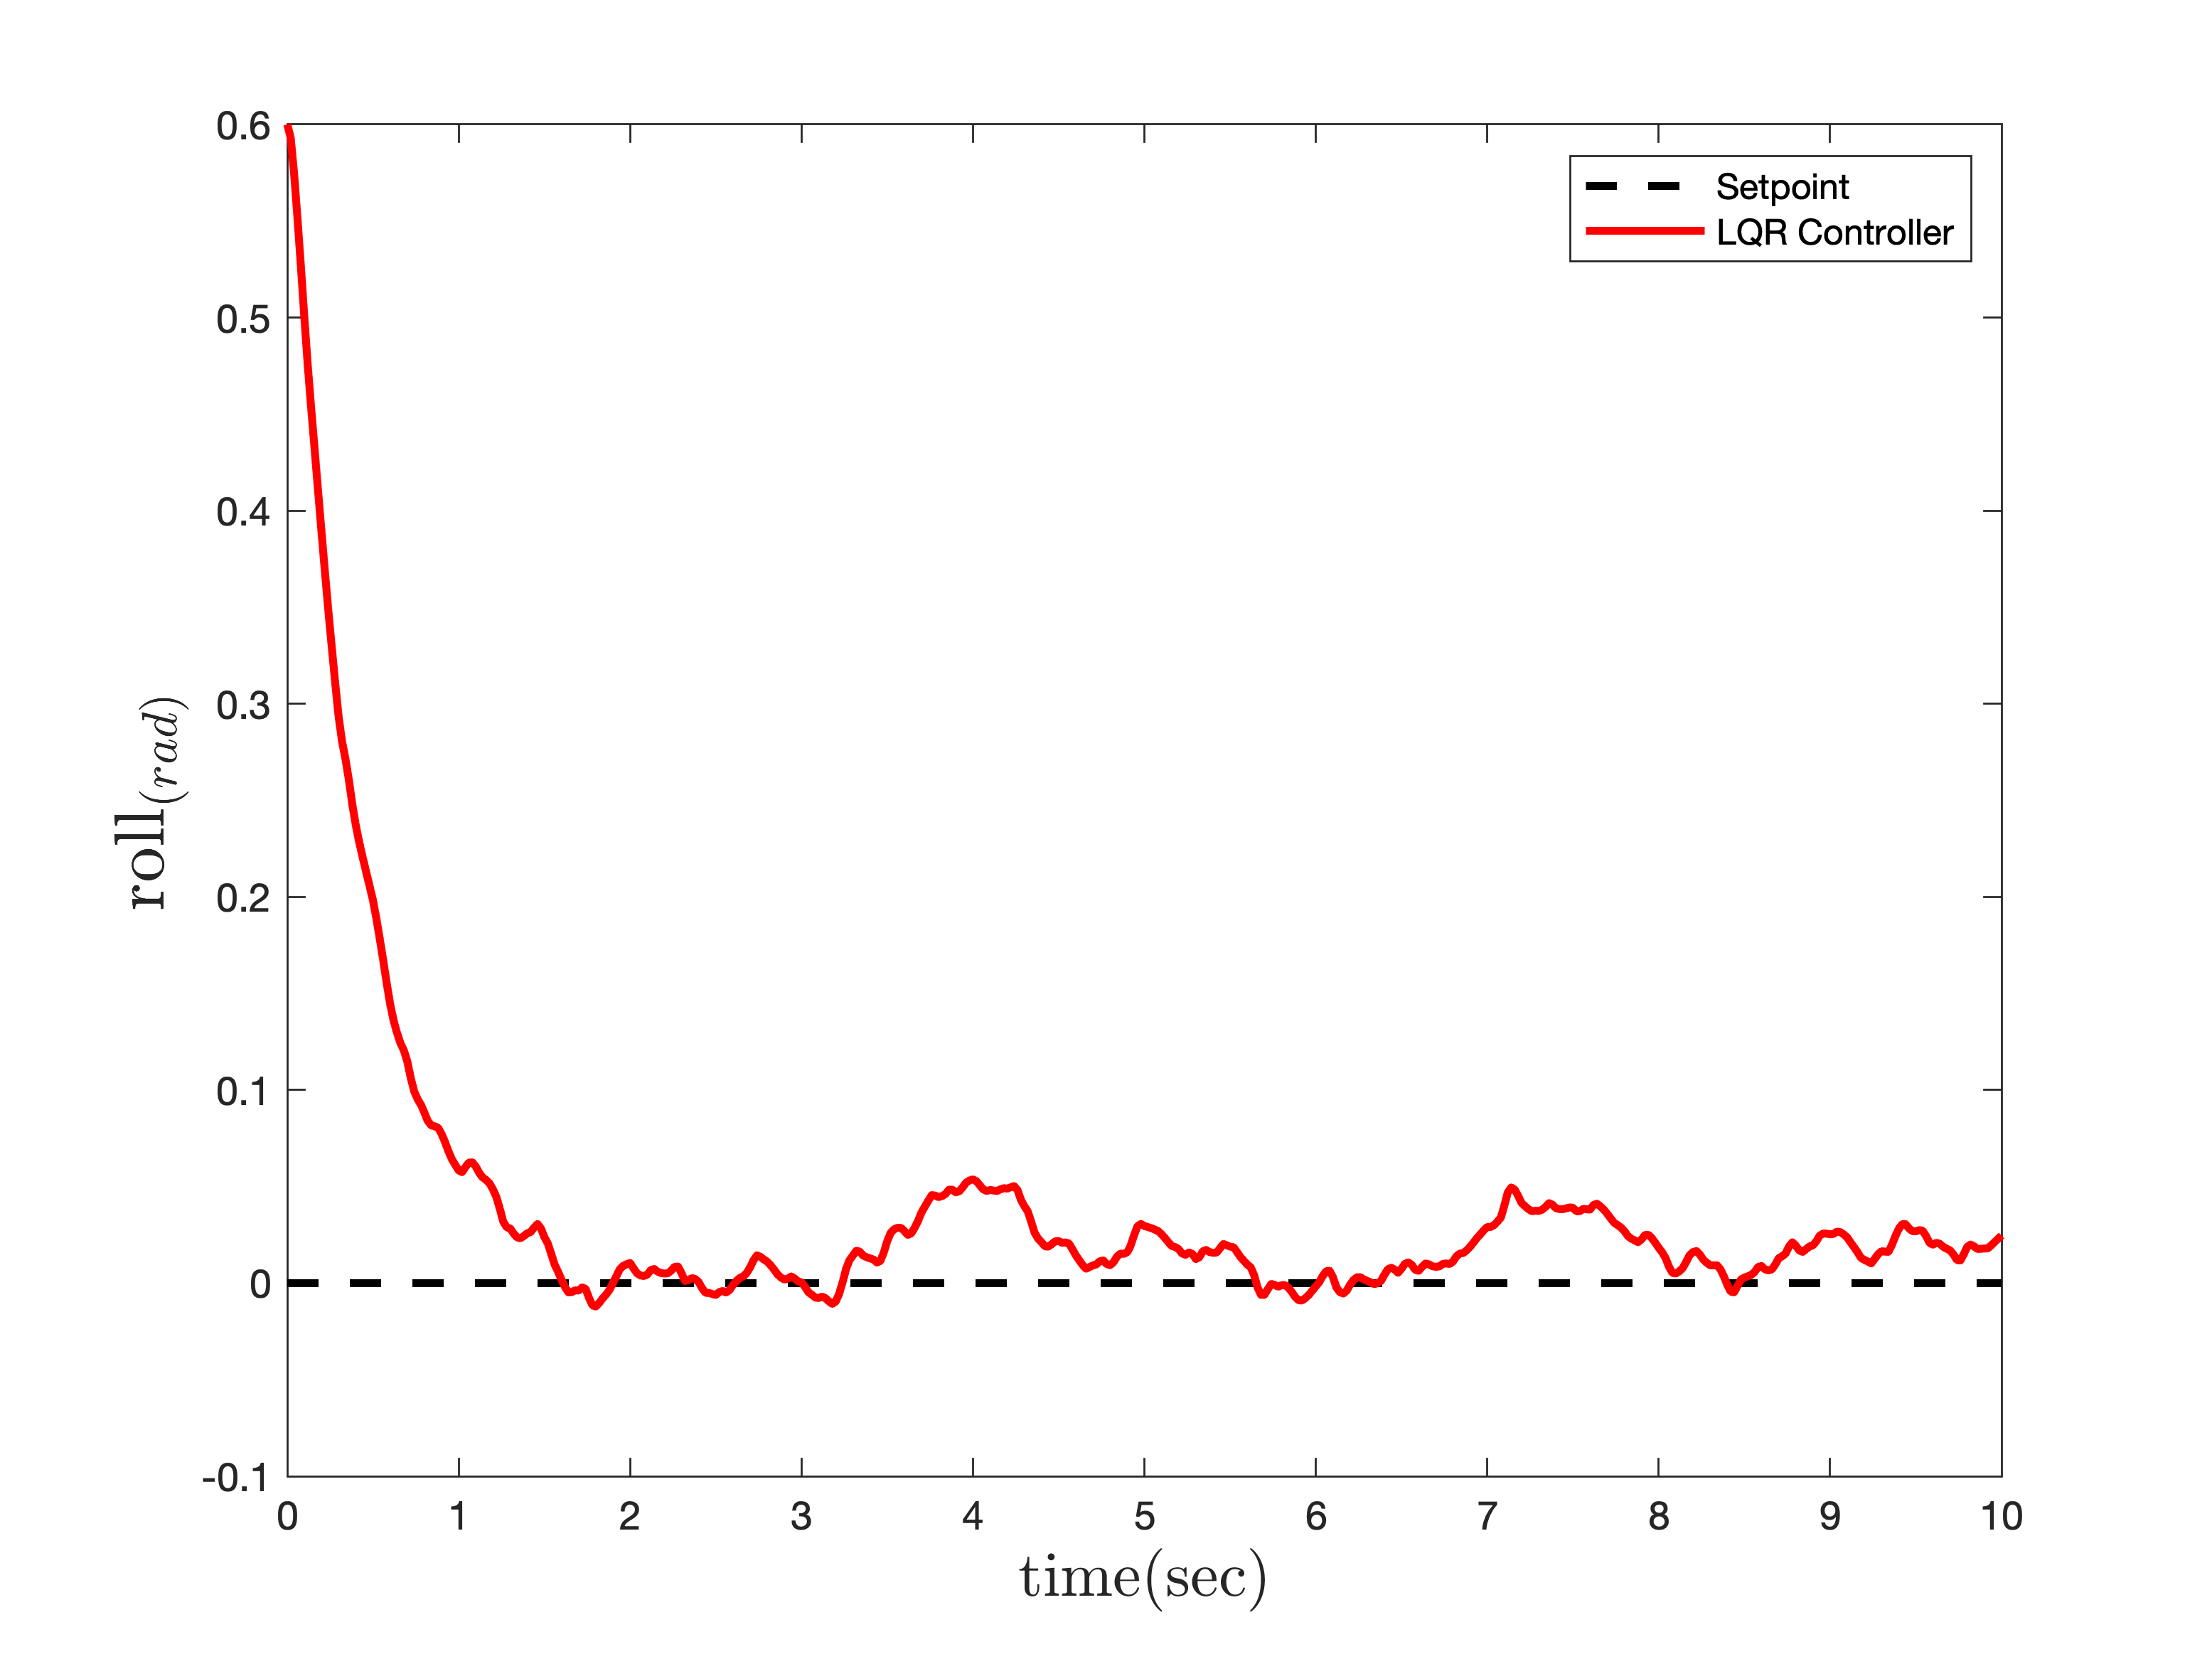
\includegraphics[width=.48\linewidth]{../Figures/MIL/LQR/Roll/lqr_roll.png}
	\centering
	\caption{عملكرد \lr{LQR} در کنترل زاويه رول (تعقیب ورودی صفر)}
	\label{lqr_roll_figure_simulation}
\end{figure}
\begin{figure}[H]
	\centering
	\subfigure[موتور شماره دو]{
		\centering
		\includegraphics[width=.45\linewidth]{../Figures/MIL/LQR/Roll/lqr_roll_Omega_2.png}
	}
	\subfigure[موتور شماره چهار]{
		\centering
		\includegraphics[width=.45\linewidth]{../Figures/MIL/LQR/Roll/lqr_roll_Omega_4.png}
	}
	\caption{‫‪فرمان کنترلی موتورها در کنترل زاویه رول (تعقیب ورودی صفر)}
\end{figure}


بر اساس خروجی شبیه‌سازی (شکل
\ref{lqr_roll_figure_simulation})،
کانال رول در حضور کنترل‌کننده \lr{LQR} در حدود پنج ثانیه به تعادل می‌رسد اما دارای خطای ماندگار است. 